% Options for packages loaded elsewhere
\PassOptionsToPackage{unicode}{hyperref}
\PassOptionsToPackage{hyphens}{url}
%
\documentclass[
]{article}
\usepackage{amsmath,amssymb}
\usepackage{iftex}
\ifPDFTeX
  \usepackage[T1]{fontenc}
  \usepackage[utf8]{inputenc}
  \usepackage{textcomp} % provide euro and other symbols
\else % if luatex or xetex
  \usepackage{unicode-math} % this also loads fontspec
  \defaultfontfeatures{Scale=MatchLowercase}
  \defaultfontfeatures[\rmfamily]{Ligatures=TeX,Scale=1}
\fi
\usepackage{lmodern}
\ifPDFTeX\else
  % xetex/luatex font selection
\fi
% Use upquote if available, for straight quotes in verbatim environments
\IfFileExists{upquote.sty}{\usepackage{upquote}}{}
\IfFileExists{microtype.sty}{% use microtype if available
  \usepackage[]{microtype}
  \UseMicrotypeSet[protrusion]{basicmath} % disable protrusion for tt fonts
}{}
\makeatletter
\@ifundefined{KOMAClassName}{% if non-KOMA class
  \IfFileExists{parskip.sty}{%
    \usepackage{parskip}
  }{% else
    \setlength{\parindent}{0pt}
    \setlength{\parskip}{6pt plus 2pt minus 1pt}}
}{% if KOMA class
  \KOMAoptions{parskip=half}}
\makeatother
\usepackage{xcolor}
\usepackage[margin=1in]{geometry}
\usepackage{color}
\usepackage{fancyvrb}
\newcommand{\VerbBar}{|}
\newcommand{\VERB}{\Verb[commandchars=\\\{\}]}
\DefineVerbatimEnvironment{Highlighting}{Verbatim}{commandchars=\\\{\}}
% Add ',fontsize=\small' for more characters per line
\usepackage{framed}
\definecolor{shadecolor}{RGB}{248,248,248}
\newenvironment{Shaded}{\begin{snugshade}}{\end{snugshade}}
\newcommand{\AlertTok}[1]{\textcolor[rgb]{0.94,0.16,0.16}{#1}}
\newcommand{\AnnotationTok}[1]{\textcolor[rgb]{0.56,0.35,0.01}{\textbf{\textit{#1}}}}
\newcommand{\AttributeTok}[1]{\textcolor[rgb]{0.13,0.29,0.53}{#1}}
\newcommand{\BaseNTok}[1]{\textcolor[rgb]{0.00,0.00,0.81}{#1}}
\newcommand{\BuiltInTok}[1]{#1}
\newcommand{\CharTok}[1]{\textcolor[rgb]{0.31,0.60,0.02}{#1}}
\newcommand{\CommentTok}[1]{\textcolor[rgb]{0.56,0.35,0.01}{\textit{#1}}}
\newcommand{\CommentVarTok}[1]{\textcolor[rgb]{0.56,0.35,0.01}{\textbf{\textit{#1}}}}
\newcommand{\ConstantTok}[1]{\textcolor[rgb]{0.56,0.35,0.01}{#1}}
\newcommand{\ControlFlowTok}[1]{\textcolor[rgb]{0.13,0.29,0.53}{\textbf{#1}}}
\newcommand{\DataTypeTok}[1]{\textcolor[rgb]{0.13,0.29,0.53}{#1}}
\newcommand{\DecValTok}[1]{\textcolor[rgb]{0.00,0.00,0.81}{#1}}
\newcommand{\DocumentationTok}[1]{\textcolor[rgb]{0.56,0.35,0.01}{\textbf{\textit{#1}}}}
\newcommand{\ErrorTok}[1]{\textcolor[rgb]{0.64,0.00,0.00}{\textbf{#1}}}
\newcommand{\ExtensionTok}[1]{#1}
\newcommand{\FloatTok}[1]{\textcolor[rgb]{0.00,0.00,0.81}{#1}}
\newcommand{\FunctionTok}[1]{\textcolor[rgb]{0.13,0.29,0.53}{\textbf{#1}}}
\newcommand{\ImportTok}[1]{#1}
\newcommand{\InformationTok}[1]{\textcolor[rgb]{0.56,0.35,0.01}{\textbf{\textit{#1}}}}
\newcommand{\KeywordTok}[1]{\textcolor[rgb]{0.13,0.29,0.53}{\textbf{#1}}}
\newcommand{\NormalTok}[1]{#1}
\newcommand{\OperatorTok}[1]{\textcolor[rgb]{0.81,0.36,0.00}{\textbf{#1}}}
\newcommand{\OtherTok}[1]{\textcolor[rgb]{0.56,0.35,0.01}{#1}}
\newcommand{\PreprocessorTok}[1]{\textcolor[rgb]{0.56,0.35,0.01}{\textit{#1}}}
\newcommand{\RegionMarkerTok}[1]{#1}
\newcommand{\SpecialCharTok}[1]{\textcolor[rgb]{0.81,0.36,0.00}{\textbf{#1}}}
\newcommand{\SpecialStringTok}[1]{\textcolor[rgb]{0.31,0.60,0.02}{#1}}
\newcommand{\StringTok}[1]{\textcolor[rgb]{0.31,0.60,0.02}{#1}}
\newcommand{\VariableTok}[1]{\textcolor[rgb]{0.00,0.00,0.00}{#1}}
\newcommand{\VerbatimStringTok}[1]{\textcolor[rgb]{0.31,0.60,0.02}{#1}}
\newcommand{\WarningTok}[1]{\textcolor[rgb]{0.56,0.35,0.01}{\textbf{\textit{#1}}}}
\usepackage{graphicx}
\makeatletter
\def\maxwidth{\ifdim\Gin@nat@width>\linewidth\linewidth\else\Gin@nat@width\fi}
\def\maxheight{\ifdim\Gin@nat@height>\textheight\textheight\else\Gin@nat@height\fi}
\makeatother
% Scale images if necessary, so that they will not overflow the page
% margins by default, and it is still possible to overwrite the defaults
% using explicit options in \includegraphics[width, height, ...]{}
\setkeys{Gin}{width=\maxwidth,height=\maxheight,keepaspectratio}
% Set default figure placement to htbp
\makeatletter
\def\fps@figure{htbp}
\makeatother
\setlength{\emergencystretch}{3em} % prevent overfull lines
\providecommand{\tightlist}{%
  \setlength{\itemsep}{0pt}\setlength{\parskip}{0pt}}
\setcounter{secnumdepth}{5}
\ifLuaTeX
\usepackage[bidi=basic]{babel}
\else
\usepackage[bidi=default]{babel}
\fi
\babelprovide[main,import]{spanish}
% get rid of language-specific shorthands (see #6817):
\let\LanguageShortHands\languageshorthands
\def\languageshorthands#1{}
\ifLuaTeX
  \usepackage{selnolig}  % disable illegal ligatures
\fi
\usepackage{bookmark}
\IfFileExists{xurl.sty}{\usepackage{xurl}}{} % add URL line breaks if available
\urlstyle{same}
\hypersetup{
  pdftitle={Eliminación de ruido en imágenes con wavelets.},
  pdfauthor={Grupo E: Alejandra Venegas, Rebeca Company, Marta Medina, Alejandro Cornelio y Ilia Zhigarev.},
  pdflang={es-ES},
  hidelinks,
  pdfcreator={LaTeX via pandoc}}

\title{Eliminación de ruido en imágenes con wavelets.}
\usepackage{etoolbox}
\makeatletter
\providecommand{\subtitle}[1]{% add subtitle to \maketitle
  \apptocmd{\@title}{\par {\large #1 \par}}{}{}
}
\makeatother
\subtitle{Análisis de señales}
\author{Grupo E: Alejandra Venegas, Rebeca Company, Marta Medina,
Alejandro Cornelio y Ilia Zhigarev.}
\date{2025-01-04}

\begin{document}
\maketitle

{
\setcounter{tocdepth}{3}
\tableofcontents
}
\section{Introducción}\label{introducciuxf3n}

En el campo del análisis de señales, uno de los problemas es la
eliminación de ruido en imágenes digitales. Las señales, que representan
variaciones de magnitudes en el espacio y/o tiempo, a menudo están
contaminadas por ruido debido a interferencias en los procesos de
captura o transmisión. Este ruido, que puede existir de formas muy
diversas como ruido gaussiano, artefactos asociados a frecuencias altas
o bajas, o efectos multiplicativos, complica la extracción de
características significativas.

El uso de wavelets es una herramienta clave para abordar este problema,
el cual permite descomponer señales en sus componentes espaciales y
frecuenciales de forma eficiente. Este método ofrece la posibilidad de
adaptarse a las características particulares de cada tipo de ruido.

En este trabajo se propone explorar la capacidad de los wavelets para la
eliminación de ruido en imágenes digitales. Para ello, se generarán y
analizarán diferentes tipos de ruido artificial, evaluando su
complejidad para su atenuación y determinando los parámetros más
eficaces de los wavelets.

\section{Fundamento teórico: eliminación de ruido con
wavelets}\label{fundamento-teuxf3rico-eliminaciuxf3n-de-ruido-con-wavelets}

Los wavelets son funciones matemáticas que permiten descomponer una
señal en componentes de diferentes escalas, lo que resulta útil para
identificar y procesar características específicas. Este enfoque es
especialmente relevante en la eliminación de ruido, donde las
frecuencias indeseadas pueden ser separadas y reducidas sin afectar
significativamente las características principales de la señal original.
A diferencia de la Transformada de Fourier, que opera globalmente y no
ofrece información sobre la localización temporal de los eventos, los
wavelets permiten un análisis localizado, facilitando la identificación
de patrones y anomalías en los datos.

El proceso de reducción de ruido con wavelets generalmente incluye tres
etapas principales: la descomposición de la señal utilizando una wavelet
madre, la modificación de los coeficientes wavelet mediante técnicas de
umbral, y la reconstrucción de la señal. La selección de la wavelet
madre adecuada y los parámetros de umbral son aspectos críticos que
deben adaptarse a las características específicas del ruido y la señal.

Además, los wavelets ofrecen un enfoque multi-resolución, permitiendo
una representación detallada de los componentes de alta frecuencia,
asociados frecuentemente con el ruido, mientras preservan las
estructuras globales de baja frecuencia. Esta característica hace que
los wavelets sean especialmente útiles en aplicaciones donde la
precisión y la integridad de los datos son esenciales, como en imágenes
médicas, procesamiento de audio o análisis de datos científicos.

En este trabajo, se emplearán wavelets como herramienta principal para
eliminar diferentes tipos de ruido sintético en imágenes.

\section{Funciones de programacion
empleadas}\label{funciones-de-programacion-empleadas}

Antes de comenzar, instalamos y/o cargamos todos los paquetes
requeridos.

Se ha escogido emplear tres métodologías distintas para realizar la
eliminación de ruido. Dos de ellas se basan en emplear la transformada
wavelet. Sin embargo, también se ha optado por emplear en un tercer
método el análisis mediante transformadas de Fourier con el objetivo de
encontrar similitudes y diferencias con respecto a los métodos que
emplean wavelets.

Con respecto a los métodos con wavelts utilizaremos un método muy
directo, empleando la función \texttt{denoise.dwt.2d} del paquete
\texttt{waveslim} de R. Por otro lado, emplearemos un método más manual
que consiste en realizar la transformada wavelet discreta con la función
\texttt{imwd}, aplicar una función para realizar el thresholding y a
continuación realizar la transformada inversa.

Para finalizar, se realizará la eliminación de ruido a través de
transformadas de Fourier con la función \texttt{fftshift} y compararemos
los resultados obtenidos con cada método.

\textbf{Método 1. Eliminación de ruido con el algoritmo de Mallat}

Empleamos la funicón \texttt{imwd()} del paquete wavethresh. Está
función realiza una transformada discreta wavelet de acuerdo con el
algoritmo de Mallat.

\begin{itemize}
\tightlist
\item
  \texttt{imwd(image,\ filter.number=10,\ family="DaubLeAsymm",\ type="wavelet",...).}
\end{itemize}

El argumento \texttt{image} de la función debe ser una matriz cuadrada
cuya dimensión sea potencia de dos.\texttt{filter.number} elige la
suavidad de la wavelet a emplear, siendo por defecto 10. \texttt{family}
indica la familia de wavelets a emplear (``DaubExPhase'' ó
``DaubLeAsymm'').Para tratar las fronteras, mantendremos el parámetro
\texttt{bc\ =\ "periodic"} por defecto.

\begin{center}\includegraphics[width=1\linewidth]{memoria_files/figure-latex/unnamed-chunk-4-1} \end{center}

Para la eliminación de ruido aplicaremos la función \texttt{threshold()}
al objeto que devuelve la función \texttt{imwd()}.

\begin{itemize}
\tightlist
\item
  \texttt{threshold(imwd,\ levels\ =\ 3:(nlevelsWT(imwd)\ -\ 1),\ type\ =\ "hard",\ policy\ =\ "universal",\ by.level\ =\ FALSE,\ value\ =\ 0,\ return.threshold\ =\ FALSE,\ compression\ =\ TRUE,\ Q\ =\ 0.05,\ ...)}
\end{itemize}

\texttt{levels} es el número de niveles a los cuáles deseamos aplicar un
umbral, mientras que \texttt{type} indica si queremos un umbral más
suave (``soft'') ó más fuerte (``hard''). El parámetro \texttt{policy}
selecciona la técnica para elegir umbral. \texttt{by.level\ =\ FALSE}
significa que se aplica un umbral global a todos los niveles indicados,
mientras que \texttt{by.level\ =\ TRUE} calcular threshold para cada
nivel por seaparado. El parámetro \texttt{value}, el valor del umbral,
se usará si elegimos técnicas manuales en \texttt{policy}. Si queremos
obtener el valor umbral aplicado, pondremos
\texttt{return.threshold\ =\ TRUE}. Finalmente, dejaremos el parámetro
\texttt{compression\ =\ TRUE} por defecto, para obterner un objeto más
pequeño.

Durante el desarrollo del trabajo variaremos estos parámetros para
observar su efecto en la eliminación de diversos tipos de ruido y
encontar aquellos que generen un mejor resultado en cada caso. Una vez
realizado el thresholding, emplearemos la función \texttt{imwr} para
realizar la transformda wavelet inversa y poder visualizar la imagen
tras la eliminación de ruido.

\textbf{Método 2. Función denoise.dwt.2d}

Empleamos la función denoise.dwt.2d del paquete waveslim para eliminar
el ruido de las imágenes empleando la transformada wavelet discreta
(DWT).

Esta función descompone la imagen en coeficientes wavelet, aplicando un
filtro wavelet seleccionado (wf) en ambos ejes (DWT-2D). Como resultado,
la imagen queda dividida en 4 cuadrantes:

\begin{itemize}
\item
  Aproximación (LL): Componentes de baja frecuencia tanto en las filas
  como en las columnas. Es la versión suavizada o ``borrosa'' de la
  imagen, que captura las características generales.
\item
  Horizontal (LH): Componentes de baja frecuencia en las filas y alta
  frecuencia en las columnas. Contiene detalles horizontales de la
  imagen.
\item
  Vertical (HL): Componentes de alta frecuencia en las filas y baja
  frecuencia en las columnas. Representa los detalles verticales (bordes
  o cambios horizontales en la imagen).
\item
  Diagonal (HH): Contiene las componentes de alta frecuencia tanto en
  las filas como en las columnas.
\end{itemize}

Esta descomposición en 4 cuadrantes se repite tantas veces como niveles
(J) se especifiquen en la función.

El siguiente paso es aplicar un umbral para ajustar o eliminar los
coeficientes de más alta frecuencia en los de cuadrantes de detalle HL,
LH y HH en cada nivel de descomposición. Cabe destacar que no se aplica
el umbral al cuadrante LL, ya que contiene las componentes de baja
frecuencia, que generalmente no están afectadas por el ruido.

Después de aplicar el umbral para suprimir el ruido, la imagen se
reconstruye empleando la transformada wavelet inversa (IDWT). Como se
observa, esta función es una aplicación más directa del método anterior,
ya implementada en una única función.

\begin{itemize}
\item
  Probaremos con dos reglas diferentes de umbral (rule):

  \begin{itemize}
  \tightlist
  \item
    hard: Anula los coeficientes por debajo del umbral, asígnándoles
    valor 0. Es una opción más agresiva.
  \item
    soft: En lugar de anular directamente los coeficientes, les otorga
    un valor gradual en función de su cercanía al umbral. Permite una
    reducción del ruido menos abrupta.
  \end{itemize}
\item
  Niveles de descomposición (J):
\end{itemize}

Probaremos tres niveles de descomposición distintos. El ruido suele
encontrarse en las altas frecuencias de los niveles más bajos, mientras
que en los niveles altos se encuentran los detalles más finos. Esperamos
que un mayor nivel de descomposición genere imágenes más suavizadas,
pero con menos detalles.

\begin{itemize}
\tightlist
\item
  Filtros wavelet:
\end{itemize}

Finalmente, realizaremos la descomposición de la imagen con 4 filtros
wavelet distintos, son 4 wavelets con diferentes formas (pueden ser
simétricas o no), y diferente numero de coeficientes.

\begin{itemize}
\tightlist
\item
  d4 (Daubechies 4),la8 (Least Asymmetric 8), bl14 (Best Localized 14),
  mb8 (Maximum Flat 8)
\end{itemize}

\textbf{Método 3. Transformada de Fourier (función fftshift)}

El método usado usa la transformada rápida de fourier para poder
eliminar altas frecuencias correspondientes a ruido en la imagen. La
función \emph{fftshift} desplaza las bajas frecuencias al centro del
espectro y las altas a los extremos. Una vez se visualiza el espectro,
se procede a disminuir la magnitud de las altas frecuencias cercanas a
los extremos asignandoles una magnitud menor. Con este procedimiento
estamos aplicando un filtro de paso bajo y aplicando \emph{ifftshift}
obtenemos la imagen en el dominio espacial con ruido eliminado.

Además, a lo largo de las funciones ya implementadas en R a lo largo del
trabajo se programaran diversas funciones que ayudarán a automatizar el
proceso.

\section{Desarrollo y resultados}\label{desarrollo-y-resultados}

Comenzamos cargando y visualizando las fotografías a emplear.

Vamos a visualizar las imágenes empleadas. Se han tomado 5 imágenes
distintas pero todas con la misma temática. La elección se ha realizado
pensando en poder observar como afecta la elimación de ruido detalles
como la textura o defectos en las frutas. Además, las imágenes 1 a 4 se
han tomado con una cámara de gran calidad, mientras que la imagen 5
cuenta con una resolución mucho menor. Se busca también estudiar que
efecto tiene la resolución de la imagen y su calidada en la eliminación
de ruido.

\begin{center}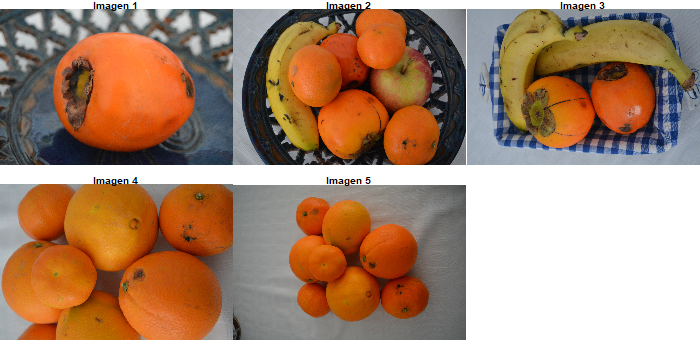
\includegraphics[width=1\linewidth]{imwd/all_images} \end{center}

\subsection{Inclusión de ruido sintético en las
imágenes}\label{inclusiuxf3n-de-ruido-sintuxe9tico-en-las-imuxe1genes}

Se crean la función \texttt{add\_noise\_to\_image} y
\texttt{NOISE\_TYPES} para añadir el ruido a las imágenes. Los ruidos
que se han generado, con parámetros ajustables a variar, son los
siguientes:

\begin{itemize}
\tightlist
\item
  Ruido gaussiano de media 0 y desviación típica ajustable.
\item
  Ruidos sinusoidales de alta y baja frecuencia.
\item
  Ruido sal y pimienta: Este tipo de ruido sustituye píxeles aleatorios
  en la imagen por valores mínimos (negros) o máximos (blancos),
  simulando un patrón de puntos oscuros y brillantes
\item
  Ruido gamma multiplicativo: multiplica el valor de los píxeles por una
  distribución gamma.
\item
  Ruido uniforme multiplicativo: multiplica el valor de los píxeles por
  una distribución uniforme.
\end{itemize}

Estos ruidos sintéticos pueden imitar ruidos que se encuentren en
imágenes reales. Por ejemplo, el ruido sinusoidal introduce un patrón
periódico de oscilaciones que pueden simular interferencias periódicas.
Otro ejemplo es el ruido sal y pimienta, que puede simular fallos en la
captura de las imágenes (la aparición de puntos blancos y negros).

\subsection{Función imwd}\label{funciuxf3n-imwd}

El uso de la Transformada Discreta de Wavelet (DWT) permite separar las
frecuencias bajas de las frecuencias altas (que son las que suelen
contener el ruido).

Uno de los parametros de la funcion explicada anteriormente (threshold)
es policy, el cual determina el valor del umbral utilizado en el proceso
de eliminación de ruido. Se exploran tres enfoques diferentes para la
selección del umbral: universal, fdr y manual.

\textbf{Umbral Universal}

El umbral ``universal'', fue propuesto por Donoho y Johnstone(1995).
Esta estrategia calcula el umbral aplicado a los coeficientes de wavelet
en función del tamaño de la señal y una estimación del nivel de ruido.
Este enfoque tiene como objetivo establecer un umbral de manera que se
eliminen los coeficientes de wavelet que corresponden al ruido, mientras
se conservan aquellos que contienen la señal significativa. La fórmula
del umbral ``universal'' es \[ \sigma \sqrt{2 \log nd}\] donde
\(\sigma\) es una estimación del ruido y \emph{nd} es el número de
coeficientes en la subbanda de detalles correspondiente a un nivel de la
transformada wavelet. Este valor se obtiene accediendo a los
coeficientes de la subbanda D de cada nivel.

\textbf{Umbral FDR}

La tasa de falsos positivos (FDR) es una técnica estadística utilizada
para controlar la tasa de falsos positivos en el proceso de selección de
coeficientes relevantes, tal como se describe en el trabajo de
Abramovich y Benjamini (1996). En el contexto de la reducción de ruido
mediante la Transformada Wavelet, el objetivo principal de FDR es
identificar y eliminar los coeficientes asociados al ruido, mientras se
preservan aquellos que contienen información significativa, como bordes,
texturas o detalles importantes de la imagen. Esto se logra calculando,
para cada coeficiente de la transformada, la probabilidad de que dicho
coeficiente sea un falso positivo, es decir, que corresponda a ruido
pero sea erróneamente considerado relevante.

\textbf{Umbral Manual}

Se fija un umbral manualmente.

\subsubsection{Redimensionando las
imágenes}\label{redimensionando-las-imuxe1genes}

Para aplicar el algoritmo de Mallat (IMWD), es necesario que la imagen
tenga una forma cuadrada cuyas dimensiones sean potencia de dos. Dado
que muchas imágenes no son cuadradas, es necesario convertirlas antes de
aplicar el algoritmo, por lo que debemos realizar un pre-procesamiento
de las imágenes. Se han escogido 2 maneras distintas para obtener
imágenes con el tamaño adecuado. Por un lado, redimensionaremos las
imágenes con la función \texttt{resize}, lo que podría conllevar
problemas de distorsión si las imágenes estaban lejos de tener
dimensiones cuadradas. Por ello, también vamos a emplear otra técnica y
rellenaremos las matrices de las imágenes con valores de 0 ó 1 hasta
alcanzar las dimensiones adecuadas.

Como ya se ha visto para poder aplicar la función \texttt{imwd()}es
necesario partir de una matriz cuadrada cuyas dimensiones sean potencia
de dos. Por ello, en primer lugar creamos una función
\texttt{resize\_imwd()} tal que dada una foto busca la submatriz
cuadrada y potencia de dos más grande posible y a continuacón
redimensiona la imagen a dicha submatriz cuadrada.

Por otro lado, también creamos una función para el post-procesamiento de
las imágenes tras la eliminación de ruido. Queremos devolverlas a su
tamaño original con el objetivo de comparar con las imágenes iniciales.

Comenzamos generando una función \texttt{procesar\_imagen\_wavelet} con
parámetros foto, tipo y policy. Esta función realiza en primer lugar la
transformada wavelet a cada uno de los tres canales de una imagen. A
continuación, se realiza el thresholding con la función threshold,
pudiendo variar de el tipo de ``hard'' a ``soft'' y el parámetro policy
(modificando adecuadamente los parámetros necesarios en la función
threshold en este último caso). Una vez realizada la eliminación de
ruido, se aplica la trasnformada wavelet inversa \texttt{imwr} para por
último reconstruir la imagen a partir de los tres canales.

\begin{Shaded}
\begin{Highlighting}[]
\NormalTok{procesar\_imagen\_wavelet }\OtherTok{\textless{}{-}} \ControlFlowTok{function}\NormalTok{(foto, }\AttributeTok{tipo =} \StringTok{"hard"}\NormalTok{, }\AttributeTok{policy =} \StringTok{"universal"}\NormalTok{) \{}
  \CommentTok{\# 1. Realizamos la transformada wavelet a cada canal}
\NormalTok{  lwd }\OtherTok{\textless{}{-}} \FunctionTok{lapply}\NormalTok{(}\DecValTok{1}\SpecialCharTok{:}\DecValTok{3}\NormalTok{, }\ControlFlowTok{function}\NormalTok{(canal) \{}
    \FunctionTok{imwd}\NormalTok{(foto[,,canal])  }
\NormalTok{  \})}
  
  \CommentTok{\# 2. Aplicamos el umbral a los coeficientes de la transformada wavelet}
\NormalTok{  lwd\_threshold }\OtherTok{\textless{}{-}} \FunctionTok{lapply}\NormalTok{(lwd, }\ControlFlowTok{function}\NormalTok{(canal\_wd) \{}
\NormalTok{    niveles }\OtherTok{\textless{}{-}}\NormalTok{ canal\_wd}\SpecialCharTok{$}\NormalTok{nlevels}
\NormalTok{    wavethresh}\SpecialCharTok{::}\FunctionTok{threshold}\NormalTok{(canal\_wd, }\AttributeTok{levels =} \DecValTok{3}\SpecialCharTok{:}\NormalTok{(niveles}\DecValTok{{-}1}\NormalTok{), }\AttributeTok{type =}\NormalTok{ tipo,}
                          \AttributeTok{policy =}\NormalTok{ policy,}\AttributeTok{by\_level=}\ConstantTok{TRUE}\NormalTok{,}\AttributeTok{compression=}\ConstantTok{FALSE}\NormalTok{)}
\NormalTok{  \})}
  \CommentTok{\# 3. Aplicamos la transformada wavelet inversa a cada canal umbralizado}
\NormalTok{  ilwd }\OtherTok{\textless{}{-}} \FunctionTok{lapply}\NormalTok{(lwd\_threshold, }\ControlFlowTok{function}\NormalTok{(canal\_umbralizado) \{}
\NormalTok{    wavethresh}\SpecialCharTok{::}\FunctionTok{imwr}\NormalTok{(canal\_umbralizado)  }\CommentTok{\# Transformada wavelet inversa}
\NormalTok{  \})}
  
  \CommentTok{\# 4. Reconstruir la imagen combinando los tres canales procesados}
\NormalTok{  imagen\_reconstruida }\OtherTok{\textless{}{-}}\NormalTok{ abind}\SpecialCharTok{::}\FunctionTok{abind}\NormalTok{(ilwd[[}\DecValTok{1}\NormalTok{]], ilwd[[}\DecValTok{2}\NormalTok{]], ilwd[[}\DecValTok{3}\NormalTok{]], }\AttributeTok{along =} \DecValTok{3}\NormalTok{)}
\NormalTok{    imagen }\OtherTok{\textless{}{-}} \FunctionTok{Image}\NormalTok{(imagen\_reconstruida, }\AttributeTok{colormode =} \StringTok{\textquotesingle{}Color\textquotesingle{}}\NormalTok{)}
  
  \FunctionTok{return}\NormalTok{(imagen)}
\NormalTok{\}}
\end{Highlighting}
\end{Shaded}

Para comenzar el análisis, vamos a emplear dos imágenes muy parecidas
(imágenes 4 y 5). Una de ellas tiene muy alta resolución mientras que la
segunda cuenta con una calidad mucho menor. El objetivo es determinar si
la resolución de la imagen afecta a la hora de eliminar ruido de esta.
Vamos a probar con el primer tipo de ruido, ruido gaussiano.

Aplicamos la función \texttt{resize\_imwd} creada anteriormente para
obtener una matriz con las dimensiones necesarias para aplicar la
transformada wavelet.

Una vez tenemos las imágenes con ruido generadas y redimensionadas
adecuadamente, podemos aplicar la función \texttt{imwd} a cada uno de
los tres canales (R, G y B). Empleamos la función
\texttt{procesar\_imagen\_wavelet} que devuelve las imágenes
reconstruidas después del thresholding. Para ruido gaussiano y para
comenzar, vamos a elegir los parámetros por defecto de la función para
el thresholding.

Finalmente, visualizamos los resultados. Primeramente, observamos las
imágenes redimensionadas con ruido y la imagen obtenida tras el uso del
método de thresholding para la eliminación de este. Observamos una
principal diferencia entre ambas: la foto que contaba con menor
resolución presenta también el peor resultado. Aunque el ruido haya sido
eliminado, sus bordes están más difuminados y tiene muy baja calidad.

\begin{center}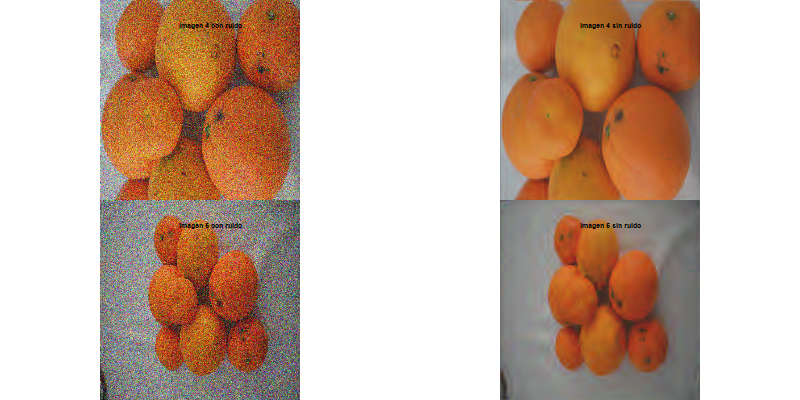
\includegraphics[width=1\linewidth]{imwd/image4_5_gaussian} \end{center}

En segundo lugar, vamos a visualizar las imágenes originales y las
imágenes sin ruido redimensionadas a su tamaño original, usando la
función \texttt{resize\_imwd\_to\_original}.

\begin{center}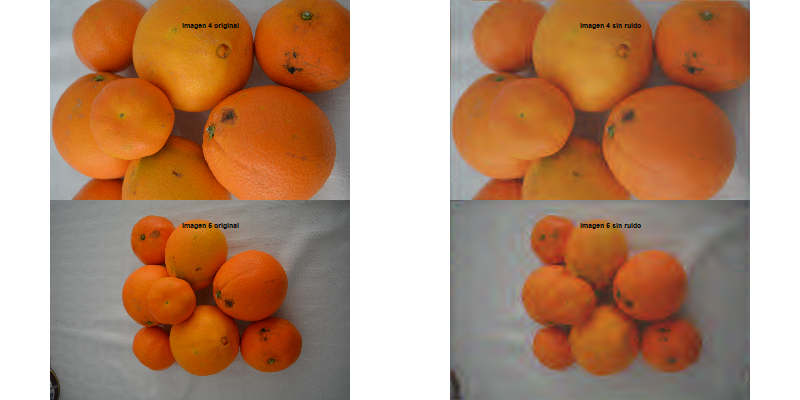
\includegraphics[width=1\linewidth]{imwd/image4_5_original_size} \end{center}

Vemos que efectivamente, la imagen que originalemente contaba con un
número de píxeles mucho menor, la imagen 5, presenta una gran distorsión
tras la eliminación de ruido.

A continuación vamos a comprobar que es lo que ocurre cuando añadimos
ruido sintético sinusoidal y si la frecuencia de este afecta al
resultado de la eliminación de ruido. Trabajaremos con una única
fotografía: la imagen 1.

Esta claro que los parámetros por defecto de la función threshold no son
capaces de eliminar el ruido de tipo sinusoidal de la manera en que si
lo era con el ruido de tipo Gaussiano, un tipo de ruido aleatorio, al
contrario que el sinusoidal, que es una señal periódica.

\begin{center}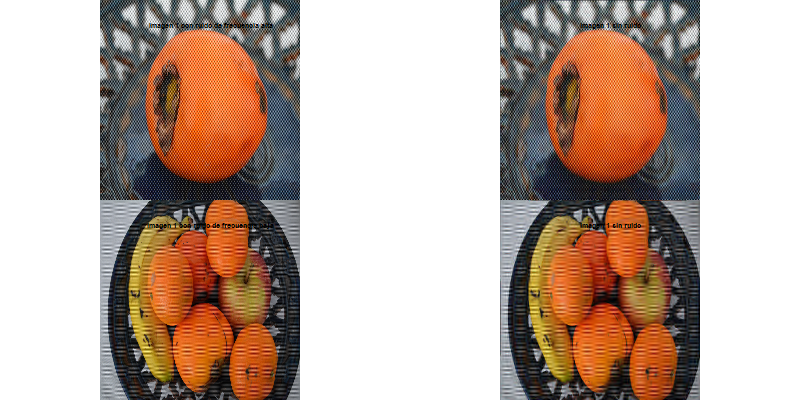
\includegraphics[width=1\linewidth]{imwd/image1_sinusoidal} \end{center}

Vamos a variar parámetros de la función threshold para intentar quitar
este ruido de manera más manual. En primer lugar, cambiamos el número de
niveles al que aplicamos el umbral, para incluirlos a todos. Cambiamos
policy a ``manual'' y variamos el valor del umbral de forma manual hasta
encontrar uno que sea satisfactorio.

Con un valor de umbral de 4 y variando el tipo a ``soft'', observamos
que hemos conseguido eliminar el ruido sinusoidal de alta frecuencia,
pero pagando un precio muy alto: los bordes de la imagen se disorsionan
completamente y tenemos una muy baja resolución. Por otro lado, el ruido
de frecuencia baja, aunque ha disminuido, claramente sigue presente en
la imagen. El umbral necesario para eliminarlo con este método es tan
alto que distorsionaría la imagen casi por completo.

\begin{center}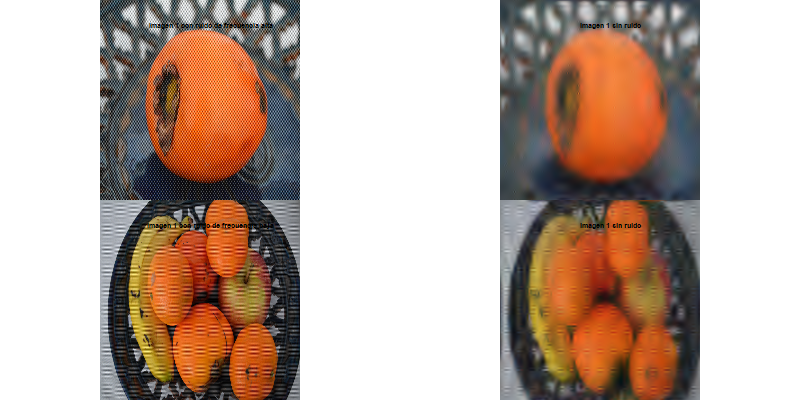
\includegraphics[width=1\linewidth]{imwd/image1_sinusoidal_manual} \end{center}

Probamos otros tipos de ruido: gamma, salt and pepper y ruido uniforme
en las imágenes 2 y 3.

Siguiendo el mismo procedimiento, redimensionamos las imágenes y y
realizamos las transformadas wavelet y el thresholding con la función
\texttt{procesar\_imagen\_wavelet}.

Visualizamos los resultados. Parece que el algoritmo funciona
correctamente para los tres tipos de ruido.

Redimensionamos las imágenes obtenidas a su tamaño original para poder
compararlas con estas. Vemos que en este caso la eliminación de ruido ha
sido bastante buena y no hay apenas distorsión ni suavizado de los
bordes.

\begin{center}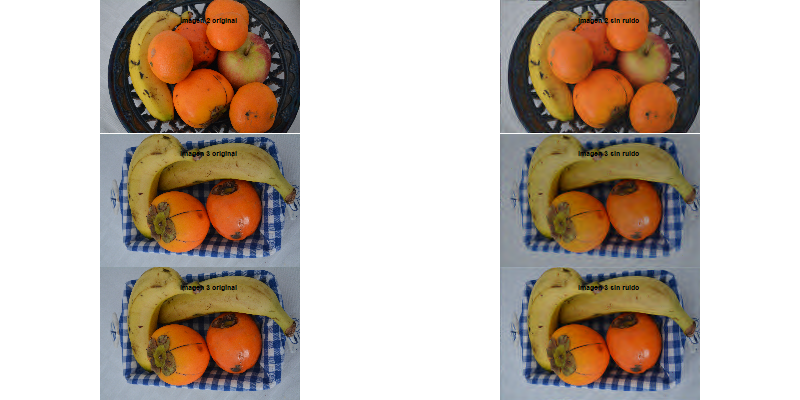
\includegraphics[width=1\linewidth]{imwd/image1_otros_ruidos_original} \end{center}

\subsubsection{Ampliando las imágenes}\label{ampliando-las-imuxe1genes}

Vamos ha emplear ahora el otro método: aumentando la matriz con 0 ó 1
hasta el tamaño adecuado para poder aplicar la función \texttt{imwd}.
Comenzamos generando las imágenes con ruido. Se elige la foto con menor
resolución (imagen 5) porque, al aplicar la función a fotos con mayor
cantidad de píxeles, se genera un problema con el uso de la memoria en R
para cargarlas debido a que la matriz se hace demasiado grande. Se
aplican distintos ruidos a la misma imagen, se presenta una foto de
ejemplo con ruido gaussiano.

Se genera una función que ajusta cualquier imagen rectangular a un
tamaño cuadrado. La diferencia con el método empleando \texttt{resize}
es que mantiene sus proporciones originales al agregar relleno si es
necesario. Esta transformación asegura que la imagen sea compatible con
el algoritmo IMWD.

Aplicamos esta función a la imagen 5 con los distintos tipos de ruido.

La imagen pasa de tener tamaño 1.600x1.066 en cada dimensión de color a
2.048x2.048, habiendo rellenado este espacio con espacio negro.

Una vez tenemos las imágenes con ruido generadas y ampliadas en potencia
de 2 en este caso de 2.048x2.048 pixeles, aplicamos la función imwd a
cada uno de los tres canales (R, G y B). Usando la función
procesar\_imagen\_wavelet que devuelve las imágenes reconstruidas
después del thresholding.

Aplicamos en cada ruido dos tecnicas para seleccionar el umbral:
Universal y fdr, además especificamos que el umbral sea `hard'.
Presentamos las imagenes sin el relleno para que sea más facil de
visualizar y ocupamos una función del paquete magick para juntar tres
imagenes y agregar título, esto lo hacemos en la función
\texttt{imprimir}.

Recordemos que la imagen 5 es la de menor resolución, por lo que, al
eliminar el ruido, los cambios no son tan notorios como en otras
imágenes.

Eliminar Ruido Gaussiano: Se observa que al eliminar el ruido gaussiano
el umbral FDR podría ofrecer una ligera mejora en la eliminación de
ruido en comparación con el umbral Universal.

\begin{center}\includegraphics[width=1\linewidth]{memoria_files/figure-latex/unnamed-chunk-48-1} \end{center}

Eliminar Ruido Sinusoidal de alta frecuencia: Al igual que en el ruido
gaussiano, se observa que al eliminar el ruido sinusoidal alto el umbral
FDR podría ofrecer una ligera mejora en la eliminación de ruido en
comparación con el umbral Universal.

\begin{center}\includegraphics[width=1\linewidth]{memoria_files/figure-latex/unnamed-chunk-49-1} \end{center}

Eliminar Ruido Sinusoidal de baja frecuencia: En este caso es muy
dificil observar diferencias

\begin{center}\includegraphics[width=1\linewidth]{memoria_files/figure-latex/unnamed-chunk-50-1} \end{center}

En los casos de ruido tipo `salt and pepper' y uniforme, se observa que
el ruido se elimina, obteniendo una imagen mejorada con FDR.

Eliminar Ruido Salt and pepper:

\begin{center}\includegraphics[width=1\linewidth]{memoria_files/figure-latex/unnamed-chunk-51-1} \end{center}

Eliminar Ruido uniforme:

\begin{center}\includegraphics[width=1\linewidth]{memoria_files/figure-latex/unnamed-chunk-52-1} \end{center}

En el caso de ruido gamma, no se logra una eliminación adecuada con FDR,
y el método universal parece ofrecer mejores resultados.

Eliminar Ruido gamma:

\begin{center}\includegraphics[width=1\linewidth]{memoria_files/figure-latex/unnamed-chunk-53-1} \end{center}

El umbral Universal emplea un valor fijo basado en el tamaño de la
señal, lo que limita su capacidad para capturar completamente la
variabilidad del ruido. En contraste, FDR estima la probabilidad de que
un coeficiente wavelet provenga del ruido, lo que le permite adaptarse
mejor a las características específicas de la señal. Como resultado, FDR
puede ofrecer una eliminación de ruido más adaptativa, preservando mejor
los detalles de la imagen. Por lo que, parece ser una opción más
adecuada en la mayoría de los casos de ruido analizados anteriormente.

\subsection{Función denoise.dwt.2d}\label{funciuxf3n-denoise.dwt.2d}

En segundo lugar, vamos a emplear la función \texttt{denoise.dwt.2d}, un
método más directo que realiza la transformada wavelet, el thresholding
y la transformada inversa en esta función ya implementada en R. A
continuación se muestran los distintos filtros wavelet que se pueden
escoger como parámetros de esta función.

Dado que se han realizado múltiples pruebas y los resultados son muy
similares, se muestran solo aquellos que se han considerado más
relevantes.

Primero, mostramos el resultado del proceso de denoising de la imagen 1,
a la que se le añadió ruido gaussiano. Este caso se utiliza como ejemplo
porque ilustra las conclusiones que también son válidas para el resto de
imágenes y tipos de ruido.

\begin{center}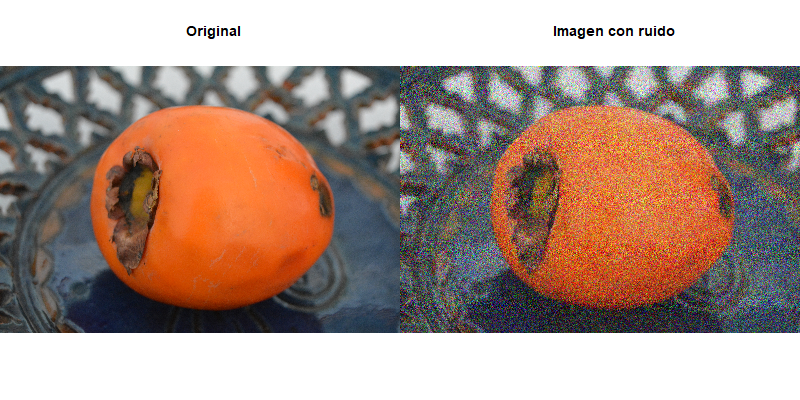
\includegraphics[width=0.4\linewidth,height=0.4\textheight]{denoisedwt2d/gaussian} \end{center}

\begin{center}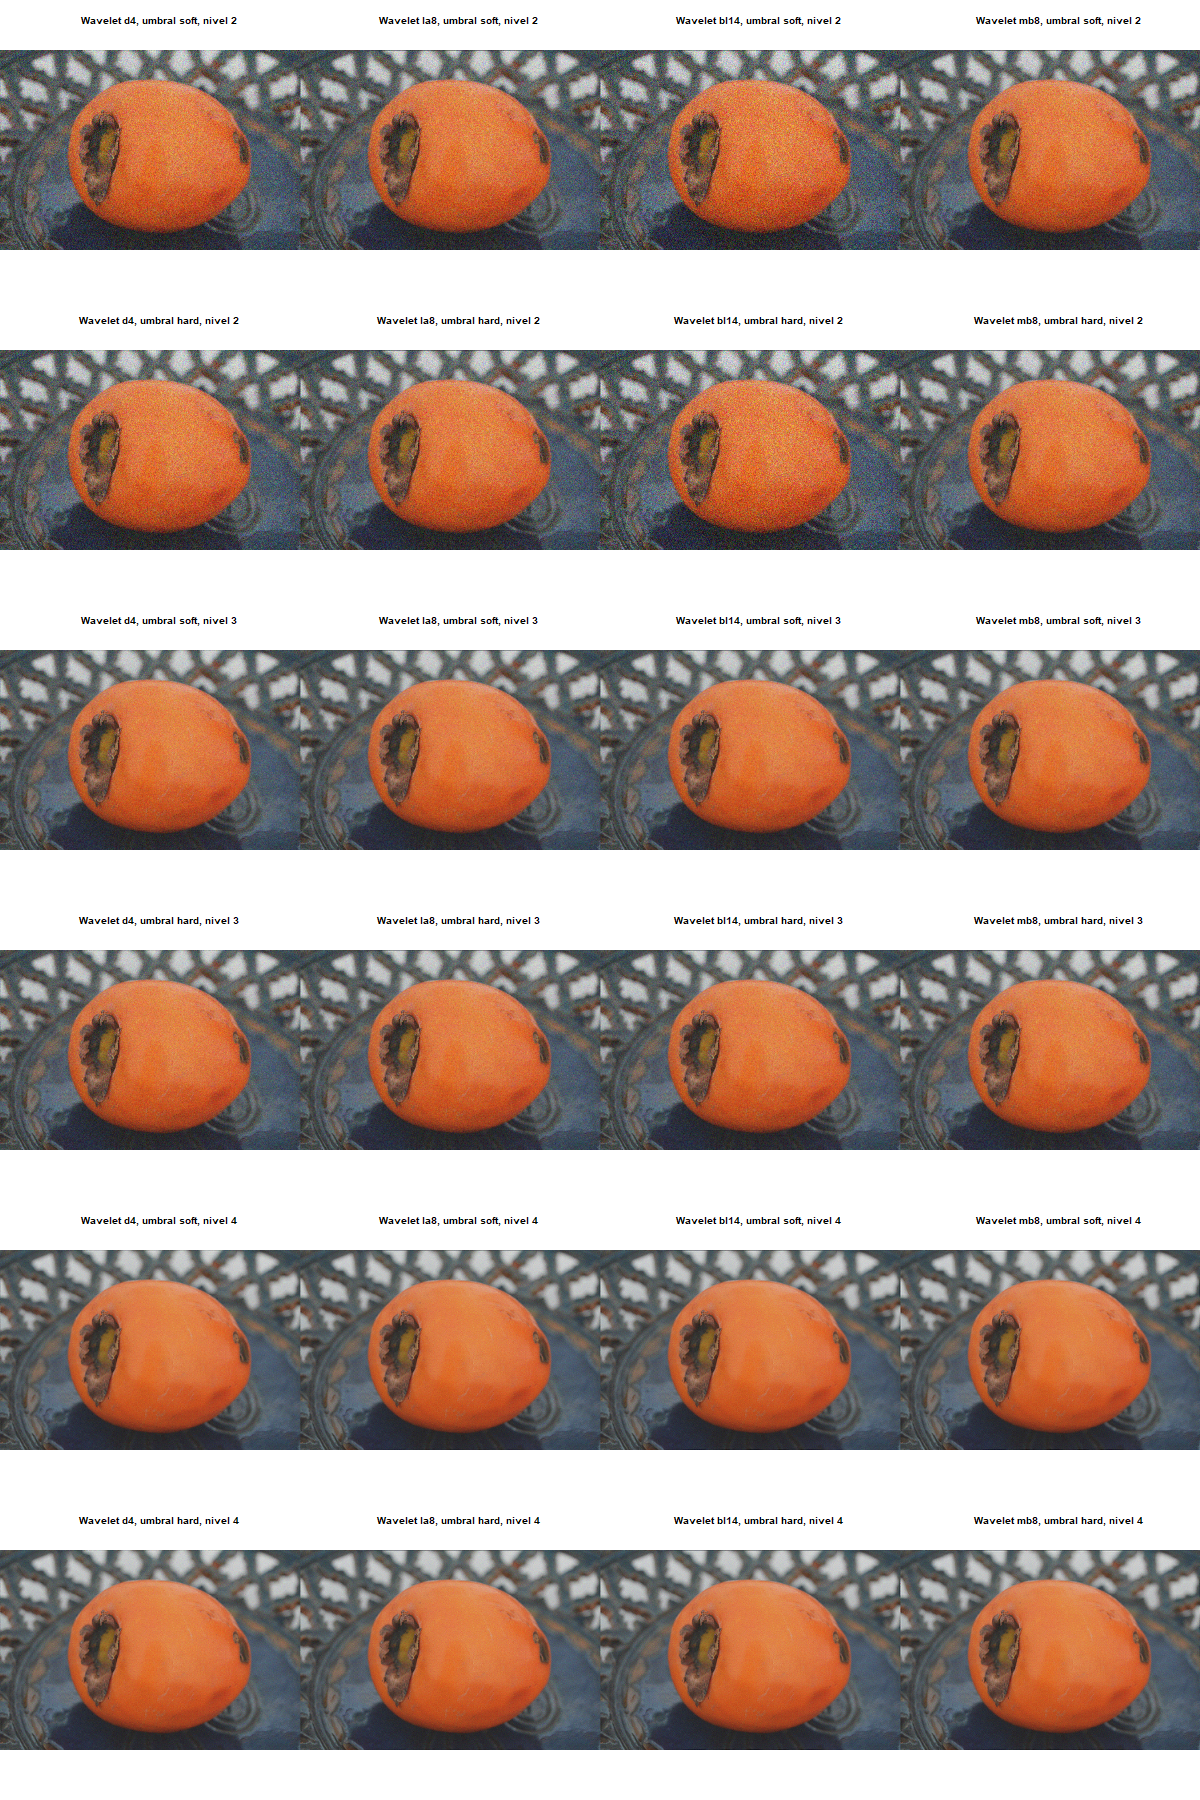
\includegraphics[width=1\linewidth]{denoisedwt2d/gaussian_denoised} \end{center}

Se observa que el uso de los diferentes filtros wavelet y reglas de
aplicación del umbral no genera resultados con diferencias
significativas. Sin embargo, el nivel de descomposición sí tiene un
impacto notable.

Con un menor número de niveles (2-3), se logran conservar los detalles
de la imagen, pero el ruido no se elimina completamente, con solo 2
niveles, el ruido sigue siendo evidente. Al aumentar a 4 niveles, se
obtiene una imagen en la que el ruido es prácticamente inapreciable,
aunque aparece algo más suavizada. Si se aumentaran aún más los niveles
de descomposición, se empezarían a perder detalles importantes de la
imagen. Con 4 niveles se consigue un buen equilibrio entre la
eliminación del ruido y la conservación de los detalles. Este
comportamiento se repite en los distintos tipos de ruido analizados.

A continuación mostramos solo algunas particularidades relevantes de los
resultados:

Por ejemplo, en el caso del ruido sinusoidal de alta frecuencia, el
resultado del proceso de eliminación de ruido es distinto.

\begin{center}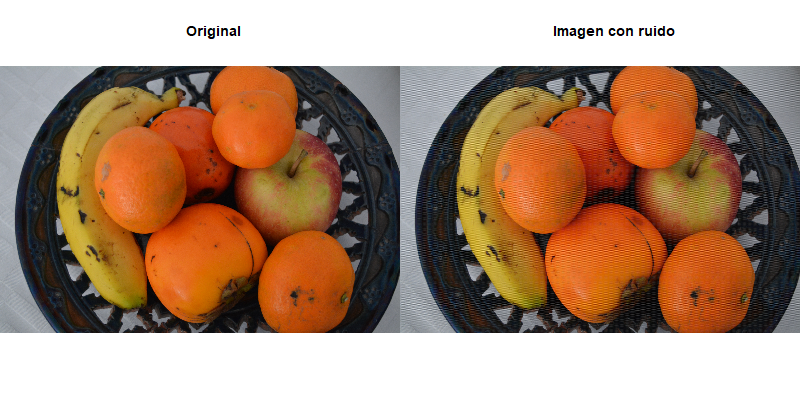
\includegraphics[width=0.5\linewidth,height=0.5\textheight]{denoisedwt2d/sinhigh} \end{center}

\begin{center}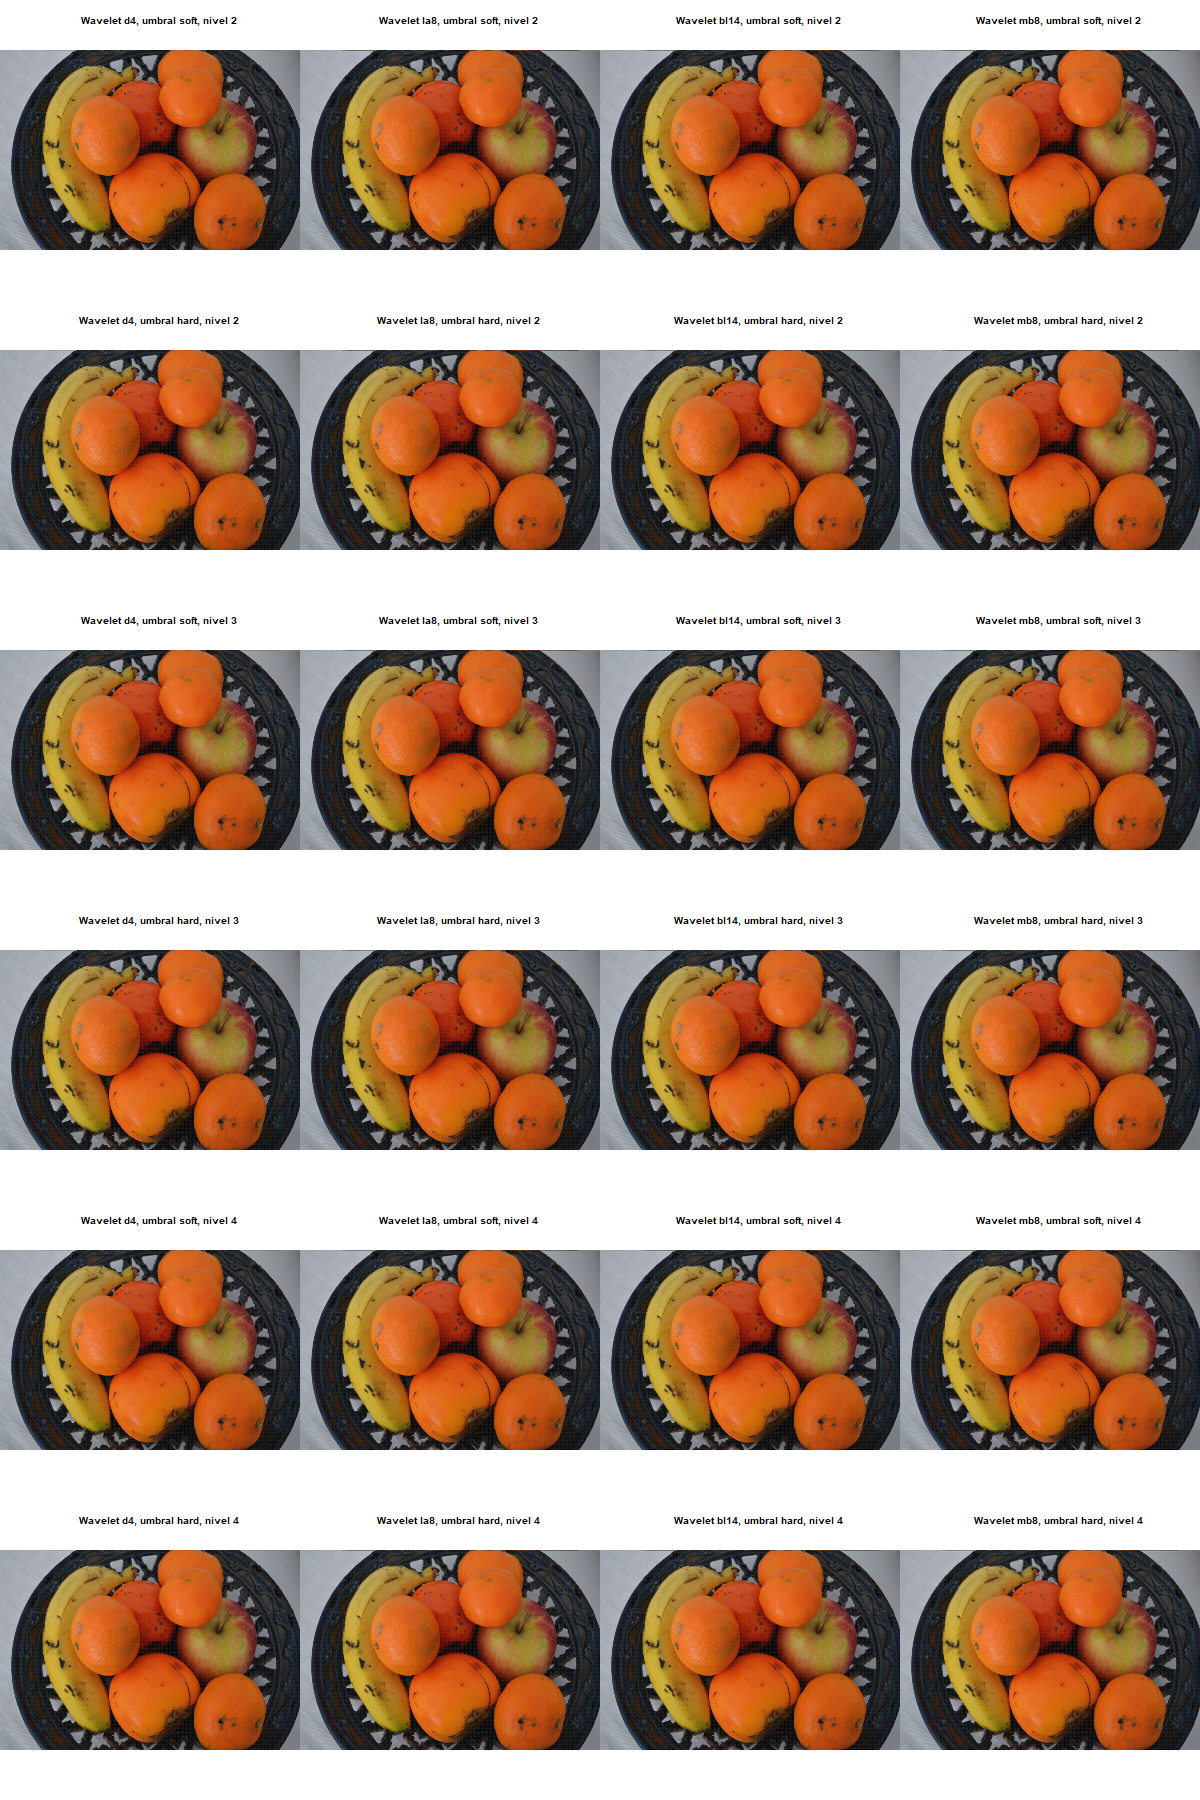
\includegraphics[width=1\linewidth]{denoisedwt2d/sinhigh_denoised} \end{center}

En este caso, vemos que en ninguno de los casos logramos eliminar
completamente el ruido sinusoidal. Esto puede deberse a que este tipo de
ruido presenta componentes muy específicas de alta frecuencia, que
pueden coincidir con las frecuencias de los detalles importantes de la
imagen, lo que dificulta eliminar el ruido sin comprometer los detalles
de la imagen. El ruido sinusoidal era también el más complicado de
eliminar cuándo aplicabamos la función \texttt{imwd} y
\texttt{threshold}.

Otro ruido que tiene resultados peculiares es el ruido de tipo
salt-and-pepper.

\begin{center}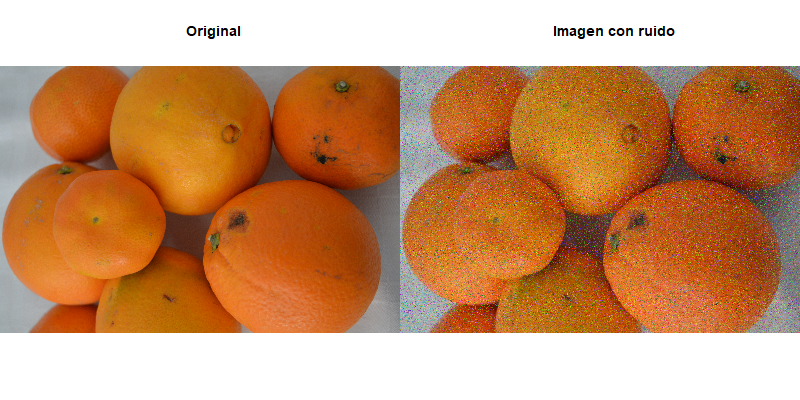
\includegraphics[width=0.5\linewidth,height=0.5\textheight]{denoisedwt2d/pepper} \end{center}

\begin{center}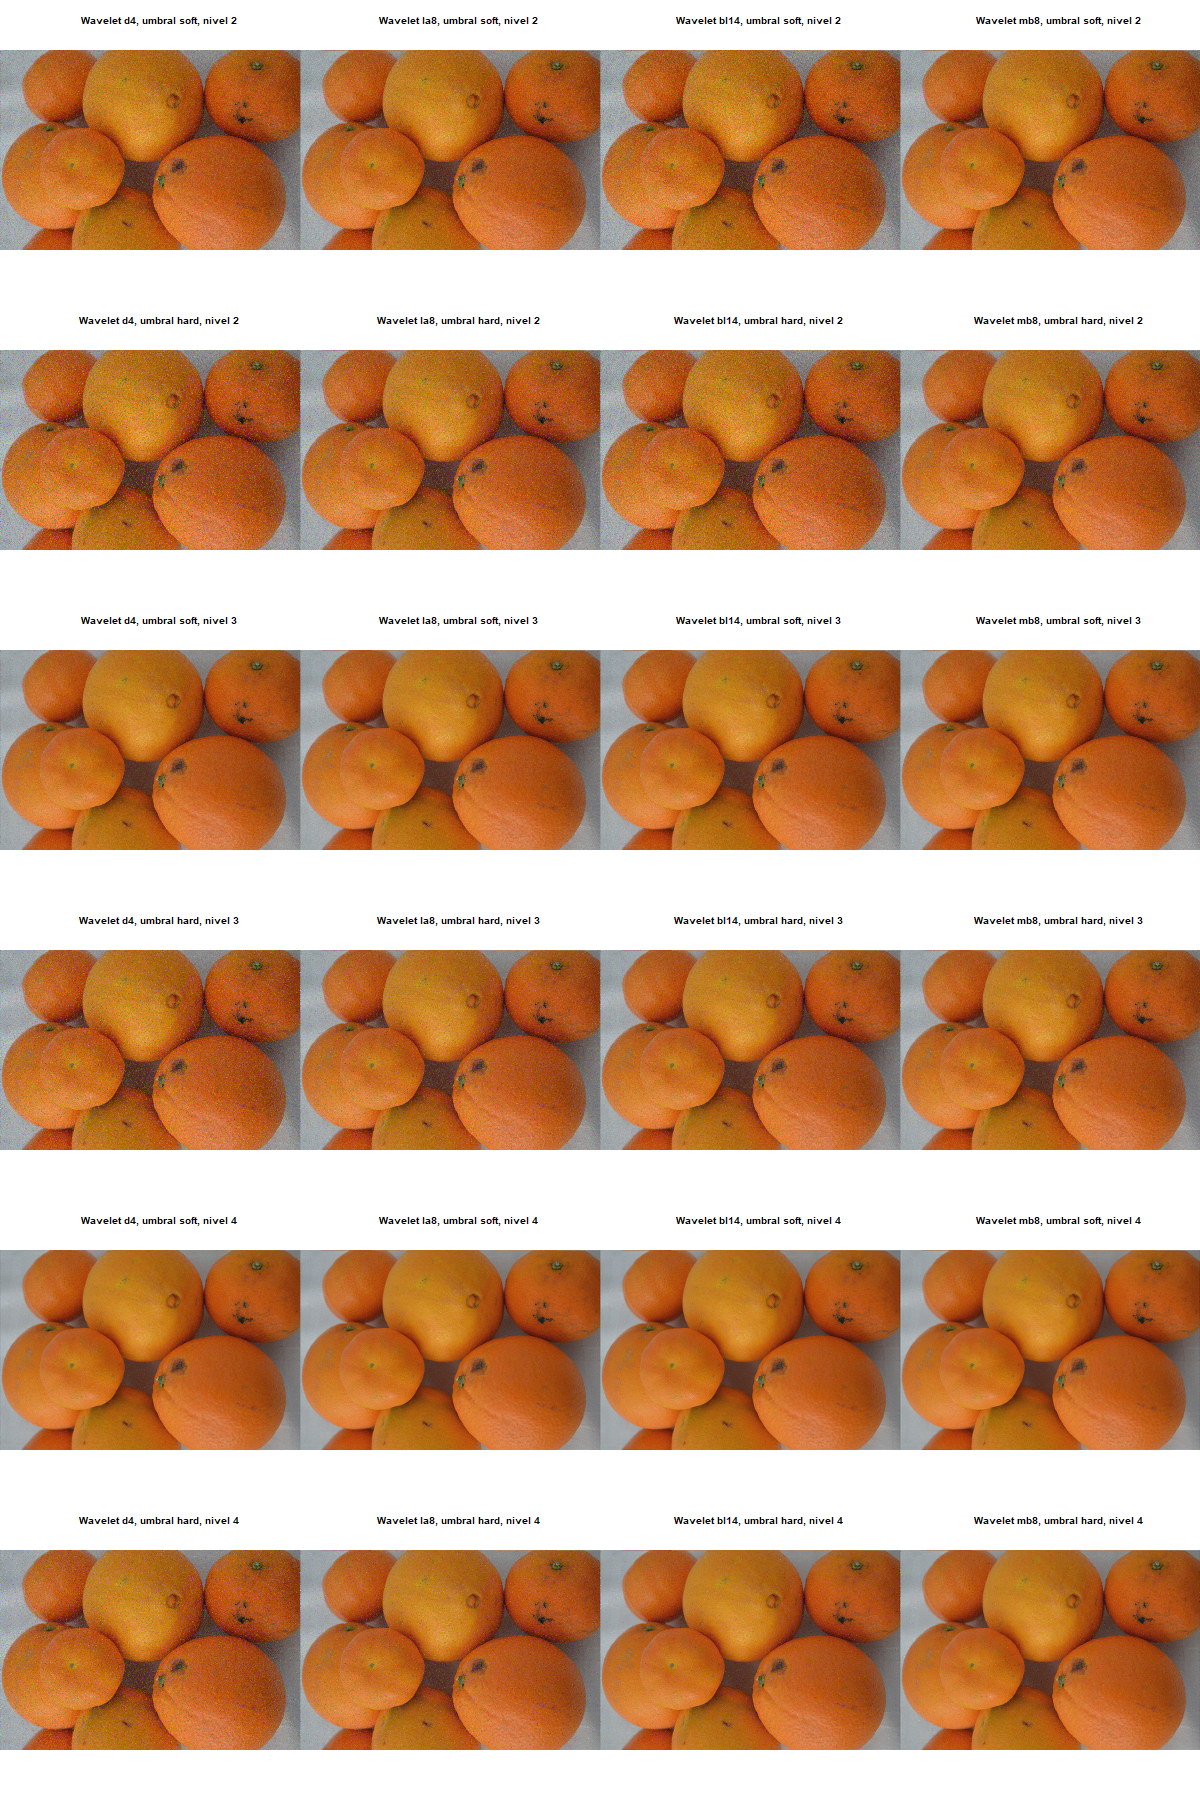
\includegraphics[width=1\linewidth]{denoisedwt2d/pepper_denoised} \end{center}

En este caso, de nuevo las diferencias más notables de deben a los
distintos niveles de descomposición, sin embargo, también observamos
diferencias sutiles en los resultados en cuanto a:

\begin{itemize}
\item
  La regla de aplicación del umbral: Al utilizar la regla soft, se
  consigue una mejor eliminación del ruido. Esto podría deberse a que el
  ruido salt and pepper asigna valores cercanos a 0 (pimienta, negro) y
  cercanos a 1 (sal, blanco) a algunos píxeles. Al aplicar el método
  hard, no se atenúan adecuadamente los picos de ruido debido a su
  naturaleza más agresiva.
\item
  El filtro wavelet empleado: El rendimiento con el filtro d4 es
  inferior al de otros filtros. Esto se debe a que el filtro d4 es un
  filtro corto (con solo 4 coeficientes) y tiene una resolución de
  frecuencia limitada. Como resultado, no puede capturar eficazmente los
  picos abruptos del ruido, como los valores 0 y 1 del ruido salt and
  pepper.
\end{itemize}

Por último, presentamos los resultados del proceso de denoising de la
imagen 5, a la que se le ha aplicado ruido gaussiano. A diferencia de la
imagen 1, en este caso la resolución de la imagen es considerablemente
inferior, lo que parece influir en los resultados obtenidos.

\begin{center}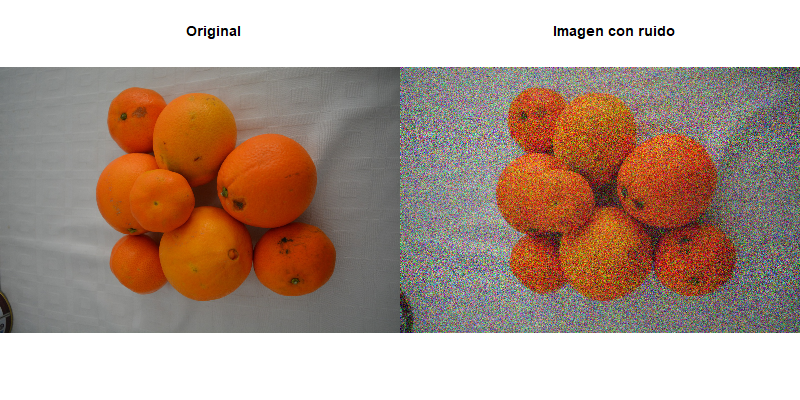
\includegraphics[width=0.4\linewidth,height=0.4\textheight]{denoisedwt2d/image5_noise} \end{center}

\begin{center}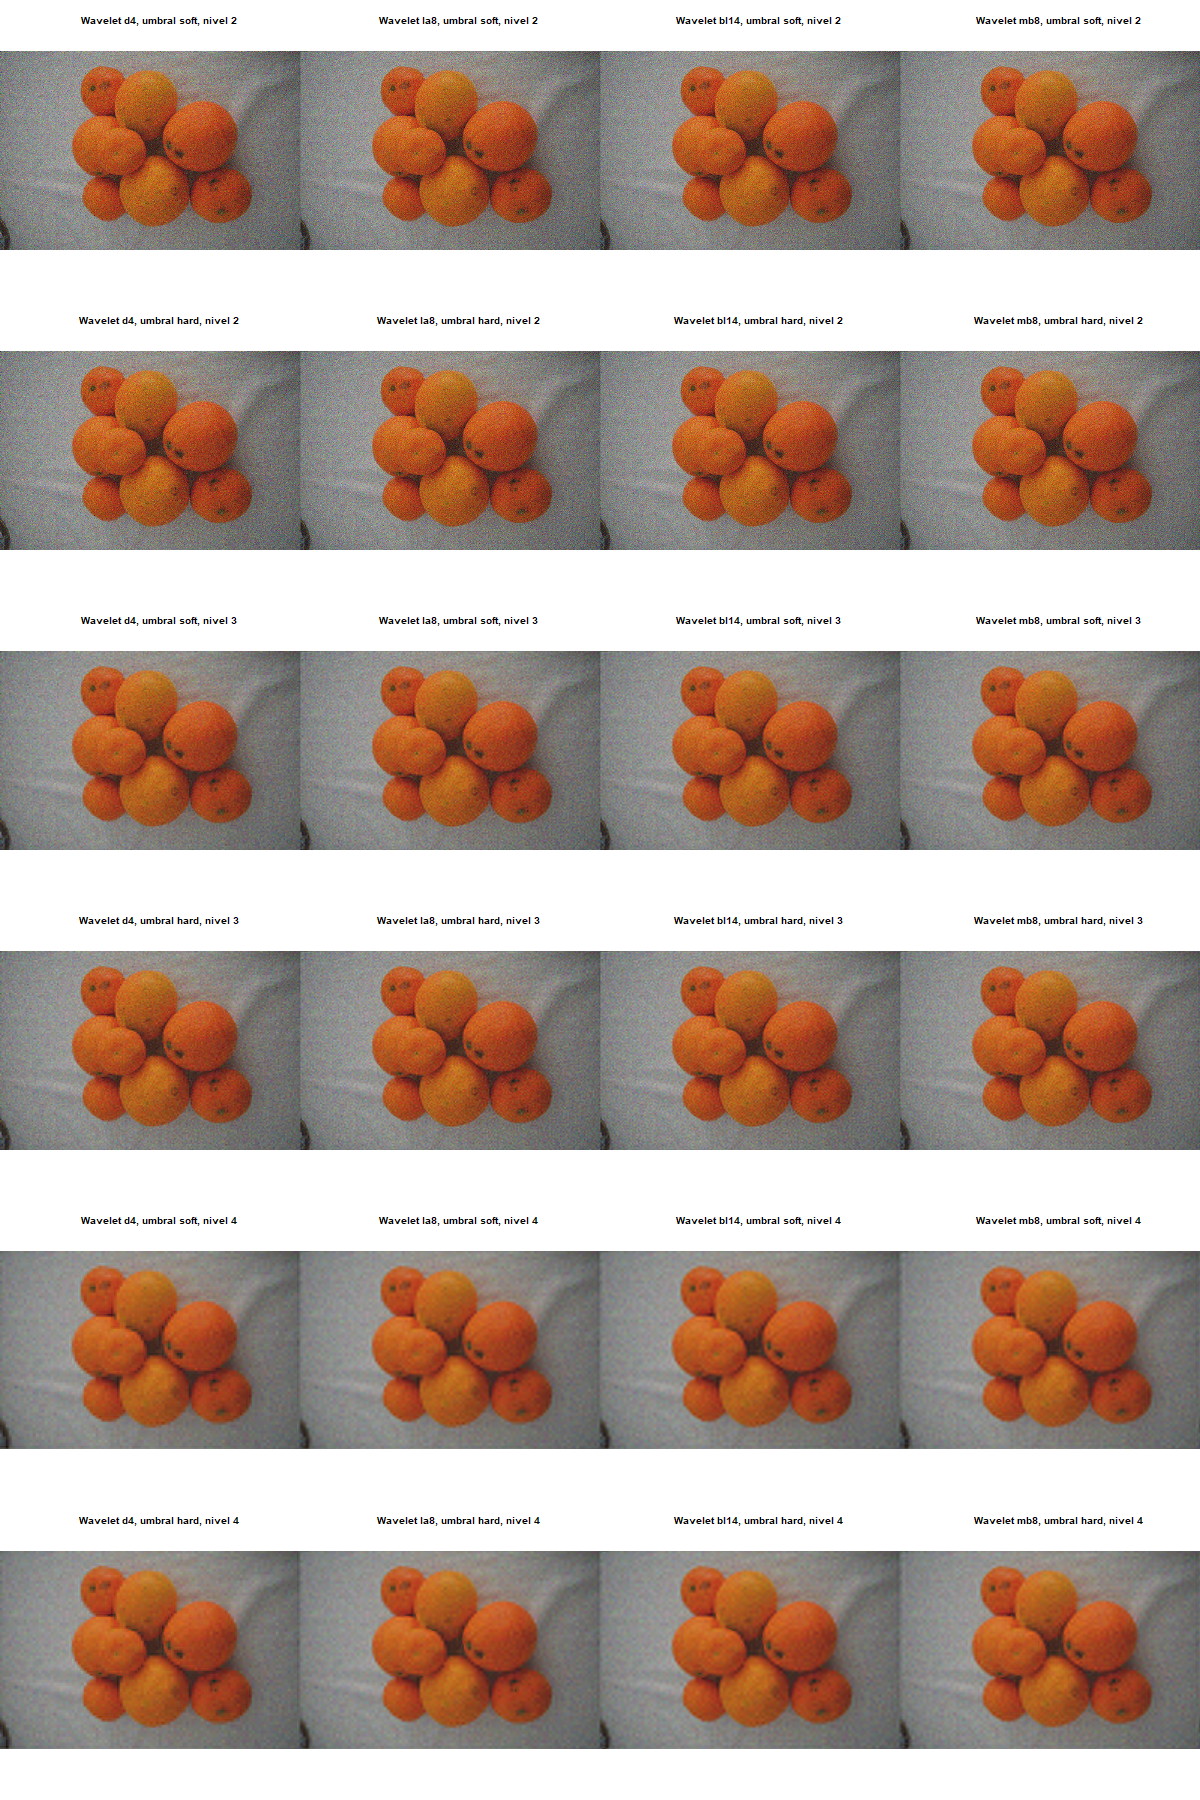
\includegraphics[width=1\linewidth]{denoisedwt2d/image5_denoised} \end{center}

La diferencia más notable en comparación con el resto de resultados, es
que en este caso, al aumentar el numero de niveles de descomposición a
un número que nos permita eliminar la mayor parte del ruido, la calidad
de la imagen se ve significativamente afectada, y obtenemos una imagen
excesivamente suavizada. Esto puede deberse a que a medida que aumentan
los niveles de descomposición, la imagen se descompone en frecuencias
cada vez más altas, provocando la pérdida de detalles finos.

La baja resolución de la imagen hace que sea más difícil mantener un
equilibrio entre la eliminación del ruido y la preservación de los
detalles. Al aumentar los niveles de descomposición, el ruido se elimina
en mayor medida, pero también se pierde mucha información útil.

\subsection{Transformada de Fourier}\label{transformada-de-fourier}

Por último, vamos a ver que es lo que ocurre cuando en lugar de
transformadas wavelet empleamos transformadas de fourier.

Comenzamos probando con la imagen 1 y el ruido gaussiano. Se realiza la
transformada de fourier y en el espacio de frecuencias se representan
las frecuencias bajas en el centro y las altas en los extremos. El
ruido, generalemente asociado a frecuencias altas, se intetará eliminar
reduciendo las frecuencias altas.

\begin{center}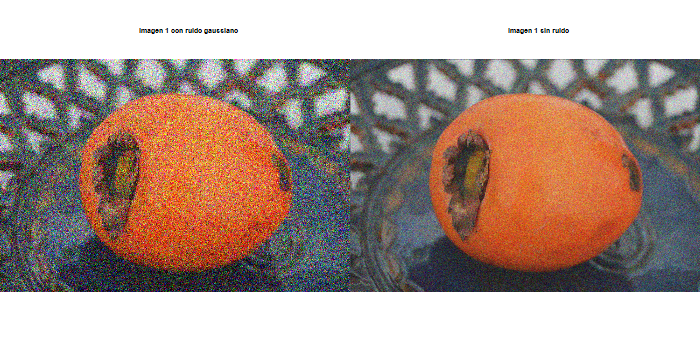
\includegraphics[width=0.4\linewidth,height=0.4\textheight]{fftshift/image1_fourier} \end{center}

La siguiente prueba se ha realizado con la imagen 2 y ruido sinusoidal
alto. Este tipo de ruido es el que más problemas generó con los otros
dos métodos.

\begin{center}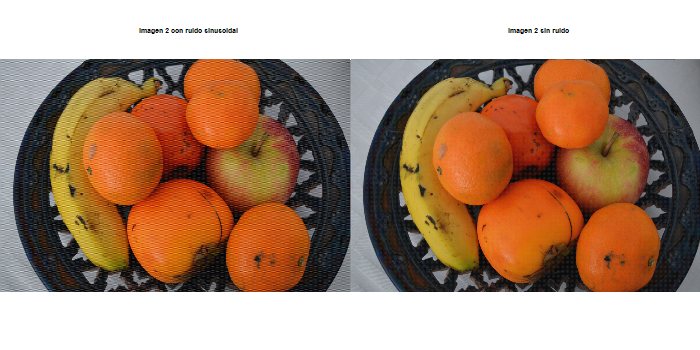
\includegraphics[width=0.4\linewidth,height=0.4\textheight]{fftshift/image2_fourier} \end{center}

\section{Conclusiones}\label{conclusiones}

\end{document}
